\documentclass[twocolumn]{extarticle}
\usepackage{fontspec}   %加這個就可以設定字體
\usepackage{xeCJK}       %讓中英文字體分開設置
\usepackage{indentfirst}
\usepackage{listings}
\usepackage[newfloat]{minted}
\usepackage{float}
\usepackage{graphicx}
\usepackage{caption}
\usepackage{fancyhdr}
\usepackage{hyperref}
\usepackage{amsmath}
\usepackage{multirow}
\usepackage[dvipsnames]{xcolor}
\usepackage{graphicx}
\usepackage{tabularx}
\usepackage{booktabs}
\usepackage{caption}
\usepackage{subcaption}
\usepackage{pifont}
\usepackage{amssymb}
\usepackage{titling}
\usepackage{physics}



\usepackage{pdftexcmds}
\usepackage{catchfile}
\usepackage{ifluatex}
\usepackage{ifplatform}

\usepackage[breakable, listings, skins, minted]{tcolorbox}
\usepackage{etoolbox}
\setminted{fontsize=\footnotesize}
\renewtcblisting{minted}{%
    listing engine=minted,
    minted language=python,
    listing only,
    breakable,
    enhanced,
    minted options = {
        linenos, 
        breaklines=true, 
        breakbefore=., 
        % fontsize=\footnotesize, 
        numbersep=2mm
    },
    overlay={%
        \begin{tcbclipinterior}
            \fill[gray!25] (frame.south west) rectangle ([xshift=4mm]frame.north west);
        \end{tcbclipinterior}
    }   
}

\usepackage[
top=1.5cm,
bottom=0.75cm,
left=1.5cm,
right=1.5cm,
includehead,includefoot,
heightrounded, % to avoid spurious underfull messages
]{geometry} 

\newenvironment{code}{\captionsetup{type=listing}}{}
\SetupFloatingEnvironment{listing}{name=Code}
\usepackage[moderate]{savetrees}


\title{NYCU Introduction to Machine Learning, Homework 4}
\author{110550088 李杰穎}
\date{}


\setCJKmainfont{Noto Serif TC}


\ifwindows
\setmonofont[Mapping=tex-text]{Consolas}
\fi

\XeTeXlinebreaklocale "zh"             %這兩行一定要加,中文才能自動換行
\XeTeXlinebreakskip = 0pt plus 1pt     %這兩行一定要加,中文才能自動換行

\setlength{\parindent}{0em}
\setlength{\parskip}{2em}
\renewcommand{\baselinestretch}{1.25}
\setlength{\droptitle}{-7.5em}   % This is your set screw
\setlength{\columnsep}{2em}
\usepackage{enumitem}

\begin{document}

\maketitle

\section{Part. 1, Coding}
\subsection{Support Vector Machine}
\begin{enumerate}
\item Show the accuracy score of the testing data using \texttt{linear\_kernel}. Your accuracy score should be higher than 0.8.

As in \autoref{fig:acc}. I set $C=4$ and achieve the accuracy of 0.83.

\item Tune the hyperparameters of the \texttt{polynomial\_kernel}. Show the accuracy score of the testing data using \texttt{polynomial\_kernel} and the hyperparameters you used.

As in \autoref{fig:acc}. I set $C=1$ and $\text{degree}=3$. In addition, the positive constant $c$ is set to 1. Under this setting, the accuracy is 0.98.

\item Tune the hyperparameters of the \texttt{rbf\_kernel}. Show the accuracy score of the testing data using \texttt{rbf\_kernel} and the hyperparameters you used.

As in \autoref{fig:acc}. I set $C=1$ and $\gamma=0.5$. The accuracy is 0.98.

\begin{figure}[H]
\centering
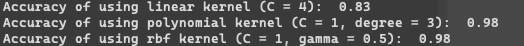
\includegraphics[width=0.95\linewidth]{acc}
\caption{The accuracy of using different kernel functions. The hyperparameters are shown in the screenshot.}
\label{fig:acc}
\end{figure}



\end{enumerate}










\section{Part. 2, Questions}


\begin{enumerate}
\item Given a valid kernel \( k_1(\mathbf{x}, \mathbf{x}') \), prove that the following proposed functions are or are not valid kernels. If one is not a valid kernel, give an example of \( k(\mathbf{x}, \mathbf{x}') \) that the corresponding \( K \) is not positive semidefinite and shows its eigenvalues.

\begin{enumerate}[label=\alph*.]
    \item \( k(\mathbf{x}, \mathbf{x}') = k_1(\mathbf{x}, \mathbf{x}') + \exp(\mathbf{x}^\top \mathbf{x}') \)
    
    We first prove that $k_2(\mathbf{x}, \mathbf{x}') = \mathbf{x}^\top \mathbf{x}'$ is a valid kernel. Suppose the basis function $\phi(\mathbf{x})=\mathbf{x}$, it's clear that the corresponding kernel function is $k_2(\mathbf{x}, \mathbf{x}')$. Therefore, $k_2$ is a valid kernel.
    
    Second, by utilizing (6.16), $\exp(\mathbf{x}^\top \mathbf{x}')$ is also a valid kernel.
    
    Lastly, by utilizing (6.17), we can finally prove that $ k(\mathbf{x}, \mathbf{x}') = k_1(\mathbf{x}, \mathbf{x}') + \exp(\mathbf{x}^\top \mathbf{x}')$ is a valid kernel.
    \item \( k(\mathbf{x}, \mathbf{x}') = k_1(\mathbf{x}, \mathbf{x}') - 1 \)
    
    Suppose $\mathbf{X}=\{x_1, x_2\}$, where $x_1=(1, 1)^\top, x_2=(3, 4)^\top$ and $k_1$ is the linear kernel. The gram matrix $\mathbf{K}=\left[ \begin{array}{cc}
    1 & 6 \\
    6 & 24 \\
    \end{array} \right]$. To calculate the eigenvalue of $\mathbf{K}$, we can solve $\det(\mathbf{K}-\lambda\mathbf{I})=0$, the solutions are $\lambda=\frac{25\pm\sqrt{673}}{2}$, one of the eigenvalues is less than zero. Therefore, $\mathbf{K}$ is not positive semi-definite, leading that $k(\mathbf{x}, \mathbf{x}') = k_1(\mathbf{x}, \mathbf{x}') + \exp(\mathbf{x}^\top \mathbf{x}')$ is not a valid kernel.
    
    \item \( k(\mathbf{x}, \mathbf{x}') = \exp(\|\mathbf{x} - \mathbf{x}'\|^2) \)
    
    Suppose, $\mathbf{X}=\{x_1, x_2\}$, where $x_1=(1, 1)^\top, x_2=(3, 4)^\top$ and $k_1$ is the linear kernel. The gram matrix $\mathbf{K}=\left[ \begin{array}{cc}
        1 & \exp(13) \\
        \exp(13) & 1 \\
        \end{array} \right]$.  To calculate the eigenvalue of $\mathbf{K}$, we can solve $\det(\mathbf{K}-\lambda\mathbf{I})=0$, the solutions are $\lambda=1\pm\exp(13)$, one of the eigenvalues is less than zero. Therefore, $\mathbf{K}$ is not positive semi-definite, leading that $k(\mathbf{x}, \mathbf{x}') = \exp(\|\mathbf{x} - \mathbf{x}'\|^2)$ is not a valid kernel.
        
    \item \( k(\mathbf{x}, \mathbf{x}') = \exp(k_1(\mathbf{x}, \mathbf{x}')) - k_1(\mathbf{x}, \mathbf{x}') \)
    
    First, we can expand $\exp(k_1(\mathbf{x}, \mathbf{x}'))$ to $1+k_1(\mathbf{x}, \mathbf{x}')+\frac{k_1(\mathbf{x}, \mathbf{x}')^2}{2!}+\frac{k_1(\mathbf{x}, \mathbf{x}')^n}{n!}+\cdots$ using Taylor's expansions. Therefore, $k(\mathbf{x}, \mathbf{x}') = \exp(k_1(\mathbf{x}, \mathbf{x}')) - k_1(\mathbf{x}, \mathbf{x}') = 1+\frac{k_1(\mathbf{x}, \mathbf{x}')^2}{2!}+\frac{k_1(\mathbf{x}, \mathbf{x}')^n}{n!}+\cdots$. It's trivial that each term in the RHS is a valid kernel by (6.18) and (6.16). For the constant $1$, the eigenvalues of its corresponding gram matrix are 0 and 1. This make it also a valid kernel. Finally, by applying (6.17), we prove that $k(\mathbf{x}, \mathbf{x}') = \exp(k_1(\mathbf{x}, \mathbf{x}')) - k_1(\mathbf{x}, \mathbf{x}')$ is a valid kernel.
\end{enumerate}

\item One way to construct kernels is to build them from simpler ones. Given three possible ``construction rules'': assuming \( K_1 (\mathbf{x}, \mathbf{x}') \) and \( K_2 (\mathbf{x}, \mathbf{x}') \) are kernels then so are

\begin{itemize}
    \item[a.] (scaling) \( f(\mathbf{x})K_1 (\mathbf{x}, \mathbf{x}')f(\mathbf{x}') \), \( f(\mathbf{x}) \in \mathbb{R} \)
    \item[b.] (sum) \( K_1 (\mathbf{x}, \mathbf{x}') + K_2 (\mathbf{x}, \mathbf{x}') \)
    \item[c.] (product) \( K_1 (\mathbf{x}, \mathbf{x}')K_2 (\mathbf{x}, \mathbf{x}') \)
\end{itemize}

Use the construction rules to build a normalized cubic polynomial kernel:
\[ K(\mathbf{x}, \mathbf{x}') = \left( 1 + \left( \frac{\mathbf{x}}{\| \mathbf{x} \|} \right)^\top \left( \frac{\mathbf{x}'}{\| \mathbf{x}' \|} \right) \right)^3 \]

You can assume that you already have a constant kernel \( K_0 (\mathbf{x}, \mathbf{x}') = 1 \) and a linear kernel \( K_1 (\mathbf{x}, \mathbf{x}') = \mathbf{x}^\top \mathbf{x}' \). Identify which rules you are employing at each step.

I solve the question by following steps:

	\begin{enumerate}
	\item Scaling the linear kernel, with $f(\mathbf{x})=\frac{1}{\| \mathbf{x} \|}$
	
	\begin{equation*}
	\mathbf{x}^\top\mathbf{x'} \Rightarrow \frac{1}{\| \mathbf{x} \|}\mathbf{x}^\top\mathbf{x'}\frac{1}{\| \mathbf{x'} \|} = \left(\frac{\mathbf{x}}{\| \mathbf{x} \|}\right)^\top\left(\frac{\mathbf{x'}}{\| \mathbf{x'} \|}\right)
	\end{equation*}
	
	\item Apply the sum construction rule, with $K_1$ is a constant kernel and $K_2$ the result from last step.
	
	\begin{equation*}
	\left(\frac{\mathbf{x}}{\| \mathbf{x} \|}\right)^\top\left(\frac{\mathbf{x'}}{\| \mathbf{x'} \|}\right) \Rightarrow 1 + \left(\frac{\mathbf{x}}{\| \mathbf{x} \|}\right)^\top\left(\frac{\mathbf{x'}}{\| \mathbf{x'} \|}\right)
	\end{equation*}
	
	\item Apply the product construction rule for two times, we will get the final kernel.
	
	\begin{equation*}
	 1 + \left(\frac{\mathbf{x}}{\| \mathbf{x} \|}\right)^\top\left(\frac{\mathbf{x'}}{\| \mathbf{x'} \|}\right) \Rightarrow \left( 1 + \left(\frac{\mathbf{x}}{\| \mathbf{x} \|}\right)^\top\left(\frac{\mathbf{x'}}{\| \mathbf{x'} \|}\right)\right)^3
	\end{equation*}
	
	
	\end{enumerate}
	
\item A social media platform has posts with text and images spanning multiple topics like news, entertainment, tech, etc. They want to categorize posts into these topics using SVMs. Discuss two multi-class SVM formulations: `One-versus-one' and `One-versus-the-rest' for this task.

	\begin{enumerate}[label=\alph*.]
	\item The formulation of the method [how many classifiers are required]
	
	For `One-versus-one', an SVM is trained for every pair of classes. Therefore, to classify $N$ classes, we need $\frac{N(N-1)}{2}$ SVMs. To classify an input, we often use majority voting to decide the output category. 
	
	As for `One-versus-the-rest', one SVM is trained per class, distinguishing that class from all other classes. Therefore, to classify $N$ classes, we only need $N-1$ classifiers to classify an input. 
	

	\item Key trade offs involved (such as complexity and robustness).
	
	The complexity of `One-versus-one' is much higher when $N$ is large, compared with `One-versus-the-rest'. However, the robustness for `One-versus-one` is higher than `One-versus-the-rest` because each classifier is trained on only two classes at a time, which might make them more specialized and potentially more accurate in distinguishing between classes.
	
	\item If the platform has limited computing resources for the application in the inference phase and requires a faster method for the service, which method is better.
	
	As I mentioned earlier, we need lots of SVMs using `One-versus-one' formulation when $N$ is large. Therefore, I suggest that `One-versus-the-rest' is a better method under the circumstance.
	\end{enumerate}

\end{enumerate}

\end{document}

